%%% Template originaly created by Karol Kozioł (mail@karol-koziol.net) and modified for ShareLaTeX use

\documentclass[a4paper,11pt]{article}

\usepackage[T1]{fontenc}
\usepackage[utf8]{inputenc}
\usepackage[francais]{babel}
\usepackage{graphicx}
\usepackage{xcolor}

\renewcommand\familydefault{\sfdefault}
\usepackage{tgheros}
\usepackage[defaultmono]{droidmono}

\usepackage{amsmath,amssymb,amsthm,textcomp}
\usepackage{enumerate}
\usepackage{multicol}
\usepackage{tikz}
\usepackage{media9}

\usepackage{url}
\usepackage{animate}
\usepackage{listings}


\usepackage{geometry}
\geometry{total={210mm,297mm},
left=25mm,right=25mm,%
bindingoffset=0mm, top=20mm,bottom=20mm}

\usepackage[colorlinks=false]{hyperref}
\linespread{1.3}

\newcommand{\linia}{\rule{\linewidth}{0.5pt}}

% custom theorems if needed
\newtheoremstyle{mytheor}
    {1ex}{1ex}{\normalfont}{0pt}{\scshape}{.}{1ex}
    {{\thmname{#1 }}{\thmnumber{#2}}{\thmnote{ (#3)}}}

\theoremstyle{mytheor}
\newtheorem{defi}{Definition}

% my own titles
\makeatletter
\renewcommand{\maketitle}{
\begin{center}
\vspace{2ex}
{\huge \textsc{\@title}}
\vspace{1ex}
\\
\linia\\
\@author \hfill \@date
\vspace{4ex}
\end{center}
}
\makeatother
%%%
\usepackage{lastpage}
% custom footers and headers
\usepackage{fancyhdr}
\pagestyle{fancy}
\lhead{}
\chead{}
\rhead{}
\lfoot{Sujet TP L3 Web2}
\cfoot{}
\rfoot{Page \thepage/\pageref{LastPage}}
\renewcommand{\headrulewidth}{0pt}
\renewcommand{\footrulewidth}{0pt}
%
%%%----------%%%----------%%%----------%%%----------%%%
\usepackage{xcolor}

\colorlet{punct}{red!60!black}
\definecolor{background}{HTML}{EEEEEE}
\definecolor{delim}{RGB}{20,105,176}
\colorlet{numb}{magenta!60!black}

\lstdefinelanguage{json}{
    basicstyle=\scriptsize\ttfamily,
    numbers=left,
    numberstyle=\scriptsize,
    stepnumber=1,
    numbersep=8pt,
    showstringspaces=false,
    breaklines=true,
    frame=lines,
    backgroundcolor=\color{background},
    literate=
     *{0}{{{\color{numb}0}}}{1}
      {1}{{{\color{numb}1}}}{1}
      {2}{{{\color{numb}2}}}{1}
      {3}{{{\color{numb}3}}}{1}
      {4}{{{\color{numb}4}}}{1}
      {5}{{{\color{numb}5}}}{1}
      {6}{{{\color{numb}6}}}{1}
      {7}{{{\color{numb}7}}}{1}
      {8}{{{\color{numb}8}}}{1}
      {9}{{{\color{numb}9}}}{1}
      {:}{{{\color{punct}{:}}}}{1}
      {,}{{{\color{punct}{,}}}}{1}
      {\{}{{{\color{delim}{\{}}}}{1}
      {\}}{{{\color{delim}{\}}}}}{1}
      {[}{{{\color{delim}{[}}}}{1}
      {]}{{{\color{delim}{]}}}}{1},
}

%\begin{filecontents}{timeline.txt}
%::0x0 % coordinate system & y=e^x, repeated until last frame
%::1 % one blue curve per frame
%::2
%::3
%::4
%::5
%::6
%::7
%::8
%\end{filecontents}

\begin{document}

\title{TP - Mémo LoL (2/3)}

\author{Université Toulouse 2 - Jean Jaurès}

%\date{01/01/2014}

\maketitle

\section*{Présentation}

Dans ce TP, il est question de développer le jeu du memory en utilisant les données du jeux League Of Legends (LoL) dont la présentation du jeu est disponible \href{http://euw.leagueoflegends.com/fr}{ici}\footnote{\url{http://euw.leagueoflegends.com/fr}}. Ce jeu propose à 10 joueurs de s'affronter en 5 contre 5, chacun incarnant un champion et devant protéger une base tout en essayant de détruire la base ennemie. Riot Games\textsuperscript{\texttrademark} (l'entreprise qui a créé ce jeu) a mis à disposition une API pour récupérer les données du jeu. Notamment les données concernant les champions disponibles. Nous proposons ici de développer le jeu du memory en utilisant ces données pour que les cartes représentent des champions du jeu LoL. 

Le jeu du memory consiste à avoir un nombre paire de cartes faces cachées présentées au joueur. Celui-ci doit retrouver les paires de cartes correspondantes. Pour cela il peut retourner simultanément 2 cartes. Si celles ci correspondent (le nom du champion est le même) alors la paire reste retournée. Sinon les deux cartes sont remises faces cachées et le joueur tente de retourner une autre paire de cartes. Le jeu se terminer lorsque toutes les paires sont trouvées. \\

\textbf{Objectif de la seconde partie de ce TP : }
développer toute la partie métier de l'application avec \textit{au choix} le framework Angular 1.* ou Angular 2.* 

\begin{center}

\includegraphics[width=0.5\textwidth]{img/lol.png} \\
%
\includegraphics[width=0.05\textwidth]{img/UOL_logo.png}
\end{center}



\newpage

\section{Interface}
Reprendre l'interface développée dans la partie précédent du TP avec les frameworks CSS Bootstrap et Less
Votre plateau doit ressembler à celui ci : \\

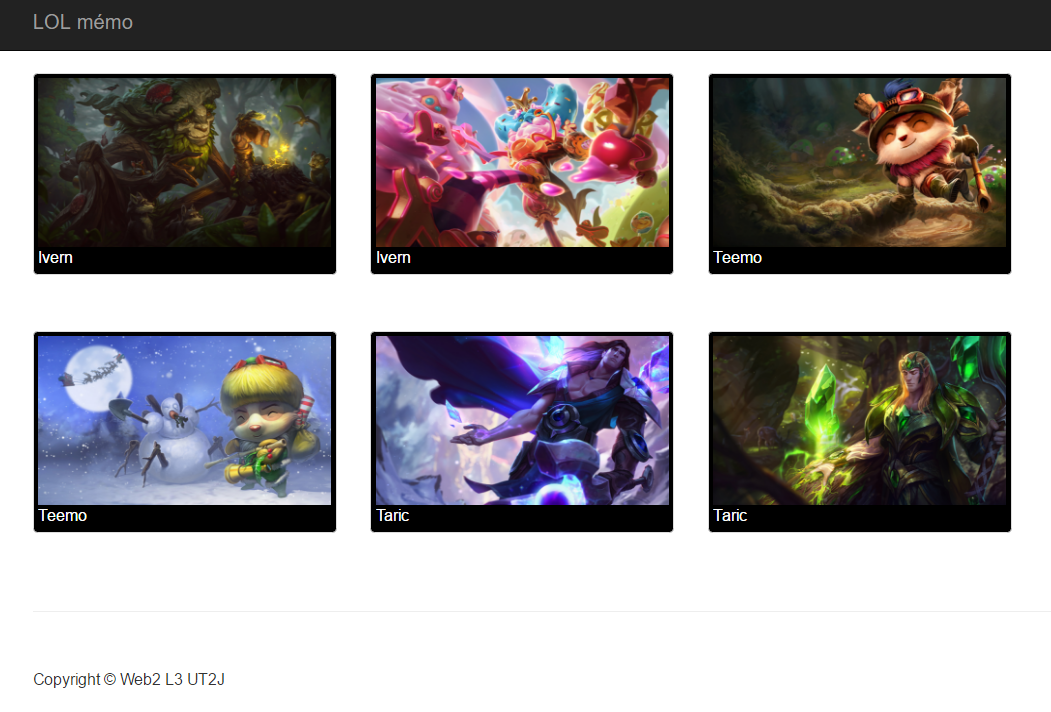
\includegraphics[width=\textwidth]{img/plateau2.png}

\section{Application}
Dans cette deuxième partie, vous devez développer toute la partie métier de l'application. Vous allez donc utiliser le framework AngularJS vu en cours pour faire ce développement. L'objectif est d'avoir le jeu du memory fonctionnel.

En utilisant l'API proposée par Riot Games\textsuperscript{\texttrademark}\footnote{\url{https://developer.riotgames.com/}} vous récupérerez les informations des champions du jeu League Of Legends. Pour cela il est nécessaire d'avoir un compte sur les serveurs de Riot. C'est le même compte que celui utilisé dans le jeu, sinon il est facile d'en créer un rapidement à cette URL : \\ \url{https://signup.euw.leagueoflegends.com/fr/signup/index?realm_key=euw} \\ Vous remarquerez que cette API propose un grand nombre de \textit{webservices} qui permettent de récupérer toutes les informations relatives au jeu, aux parties en cours et aux comptes. N'hésitez pas à explorer cette API et à proposer des idées d'applications innovantes.

\subsection{Génération aléatoire du plateau de jeu}
Jusqu'ici les champions apparaissant sur le plateau de jeu de notre memory étaient prédéterminés (Ivern, Teemo et Taric). Nous allons maintenant interroger l'API de Riot pour sélectionner 3 champions de manière aléatoire parmi tous les champions disponibles. Pour cela nous utiliserons le \textit{webservice} suivant : \\
\url{https://global.api.pvp.net/api/lol/static-data/euw/v1.2/champion?locale=fr_FR&api_key=VOTRE_CLEF }\footnote{Pensez à remplacer "VOTRE\_CLEF" par la clef fourni pour votre compte, la documentation étant disponible ici   \url{https://developer.riotgames.com/api/methods\#!/1055/3633}}\\
\begin{minipage}[h]{.45\textwidth}

Ce webservice retourne un objet JSON respectant le modèle suivant :
\begin{itemize}
    \item "data"
    \begin{itemize}
        \item nom du champion : 
        \begin{itemize}
            \item "id" : identifiant du champion
            \item "title" : titre du champion (nom long)
            \item "name" : nom du champion
            \item "key" : nom du champion en CamelCase\footnote{\url{https://fr.wikipedia.org/wiki/CamelCase}}\\ 
        \end{itemize}
    \end{itemize}
\end{itemize}
\end{minipage}
\hfill
\noindent
\begin{minipage}[h]{.45\textwidth}
\begin{lstlisting}[language=json,caption="Exemple de JSON"]
{
   "data": {
      "Aatrox": {
         "id": 266,
         "title": "the Darkin Blade",
         "name": "Aatrox",
         "key": "Aatrox"
      },
      "Thresh": {
         "id": 412,
         "title": "the Chain Warden",
         "name": "Thresh",
         "key": "Thresh"
      },
      ...
    }
}
\end{lstlisting}
\end{minipage}
\\



\normalsize

Dans cette liste vous sélectionnerez 3 champions aléatoirement et utiliserez l'attribut "key" pour obtenir les deux cartes correspondantes :
\small
\begin{itemize}
    \item \url{https://ddragon.leagueoflegends.com/cdn/img/champion/splash/{{KEY}}_0.jpg}
    \item \url{https://ddragon.leagueoflegends.com/cdn/img/champion/splash/{{KEY}}_1.jpg}
\end{itemize}
\normalsize

\subsection{Retourner une paire de cartes}
L'animation du retournement d'une carte s'effectue, jusqu'à présent, lors du survol de la souris sur celle-ci. Vous modifierez l'évènement de retournement d'une carte pour que l'animation apparaisse lors du clique de l'utilisateur sur la carte. 

De plus vous ne donnerez la possibilité de n'avoir que 2 cartes retournées en même temps. Pour cela, lorsque la deuxième carte est retournée, vous les laisserez retournées pendant 1sc\footnote{Indice : \url{https://docs.angularjs.org/api/ng/service/\$timeout\#!}} et ensuite vous retournerez ces deux cartes face cachée. Attention à ce que pendant ce temps, aucune autre carte ne puisse être retournée. 

\subsection{Déroulement de la partie}
Pour pouvoir déterminer si l'utilisateur a gagné ou non vous implémenterez les fonctionnalités du déroulement de la partie.

Tout d'abord, lorsque 2 cartes sont retournées, il faut vérifier si ces deux cartes correspondent au même champion (même "key"). Si c'est le cas alors ces deux cartes restent face visible (et ne sont donc plus cliquable). Le joueur ayant trouvé une paire, il devra trouver les autres paires du plateau.

Chaque fois qu'une paire est trouvée (2 cartes du même champion retournées) il faut vérifier s'il reste des cartes face cachée sur le plateau. Si ce n'est pas le cas alors l'utilisateur a gagné. Dans cette situation, vous afficherez un message indiquant au joueur qu'il a gagné et vous relancerez une nouvelle partie (en redéterminant les champions). 

\section{Partie bonus}
Il est possible d'améliorer ce jeu de divers manières. Il vous est proposé ici 2 améliorations que vous pouvez implémenter.
\subsection{Nombre dynamique de cartes}
Jusqu'ici le plateau contient 6 cartes en tout (2 pour les 3 champions selectionnés). Afin de déterminer le niveau de difficulté du jeu il est interessant de proposer au joueur la possibilité de choisr le nombre de carte à afficher. Ajoutez une interface avant le lancement du jeu pour demander à l'utilisateur combien de cartes il souhaite sur le plateau. 

\subsection{Calcul des points}
Il est possible de comptabiliser les points d'une partie en considérant un nombre de point initial et en décrémentant ce score pour chaque paire de carte retournée. Par exemple nous pouvons commencer la partie avec 40 points, si nous retournous 17 paires de cartes avant de trouver toutes les paires associées (et donc finir la partie), notre score sera de 23 points. Si ce score atteint 0 alors le joueur a perdu. 

\subsection{Nouvelles idées}
Comme précisez précédement, il existe de nombreuses façon d'améliorer ce jeu. Vous avez probablement plein d'idées alors n'hésitez pas à proposer de nouvelles améliorations (et aussi à les implémenter!).
\\
\\
\\

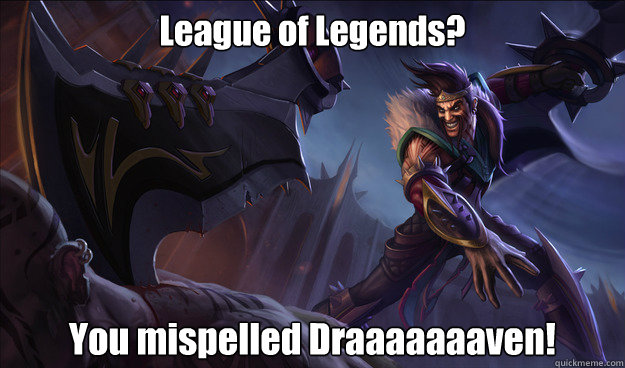
\includegraphics[width=\textwidth]{img/meme_draven.jpg}


\end{document}
